\begin{figure}[H]
\centering
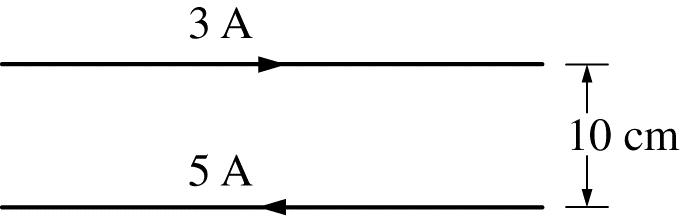
\includegraphics[scale=0.25]{images/img-009-030.png}
\end{figure}

% Multiple Choice Question 18
\begin{questions}\setcounter{question}{17}\question
Two wires are $10 \unit{cm}$ apart, as shown in the figure above. One wire has a current of 3 A to the right, and the other wire has a current of $5 \unit{A}$ to the left. What is the magnitude of the magnetic field, in teslas, at the point midway between the wires?

\begin{choices}
\choice $\dfrac{20 \times 4 \pi \times 10^{-7}}{\pi}$
\choice $\dfrac{40 \times 4 \pi \times 10^{-7}}{\pi}$
\choice $\dfrac{80 \times 4 \pi \times 10^{-7}}{\pi}$
\choice $\dfrac{100 \times 4 \pi \times 10^{-7}}{\pi}$
\choice $\dfrac{160 \times 4 \pi \times 10^{-7}}{\pi}$
\end{choices}\end{questions}

